% This file was created with tikzplotlib v0.10.1.
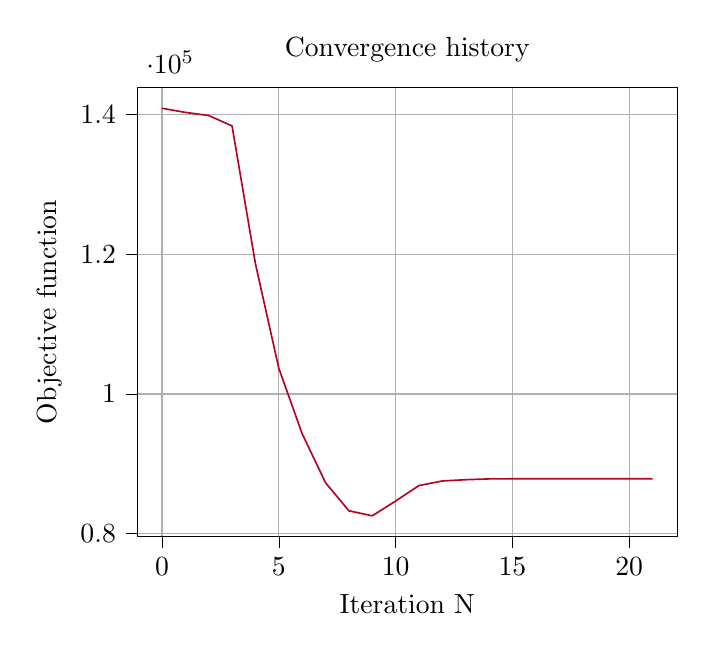
\begin{tikzpicture}

\definecolor{darkgray176}{RGB}{176,176,176}
\definecolor{firebrick180438}{RGB}{180,4,38}

\begin{axis}[
tick align=outside,
tick pos=left,
title={Convergence history},
x grid style={darkgray176},
xlabel={Iteration N},
xmajorgrids,
xmin=-1.05, xmax=22.05,
xtick style={color=black},
y grid style={darkgray176},
ylabel={Objective function},
ymajorgrids,
ymin=79642.2645959566, ymax=143829.424219743,
ytick style={color=black}
]
\addplot [semithick, firebrick180438]
table {%
0 140911.826055026
1 140318.259304388
2 139871.604737756
3 138376.671613228
4 118653.310296903
5 103698.814840816
6 94313.62886619
7 87305.8360586043
8 83281.9785556904
9 82559.8627606742
10 84668.1022357887
11 86892.8159748394
12 87547.0781509411
13 87728.5251505211
14 87843.0169232941
15 87856.8584329321
16 87857.5312890776
17 87857.6087188434
18 87857.7351359898
19 87857.8296164146
20 87857.9092345995
21 87857.9100314418
};
\end{axis}

\end{tikzpicture}
